\chapter{Implementation}

\section{Overview of Data Types}
Various new F\fsharp types have been introduced to Issie by this project. This section describes these types and provides context to them, explaining their function and the rationale behind their creation.

\subsection{Types for Representing Truth Tables}
%%%%% Commands (variables) for type information %%%%%
% Cell Table Data
\newcommand{\ttCellData}{
    Discriminated Union type representing what data each truth table cell can hold. Cells can hold Bits (represented by Issie's WireData type), Algebraic expressions (represented by strings), or a Don't Care.
}

% Cell Table Data
\newcommand{\ttCellIO}{
    Discriminated Union type representing which input or output of the logic the data belongs to. \codestyle{CellIO}s can either be the existing \codestyle{SimulationIO} type used to describe Inputs and Outputs, or Viewers.
}

% TT Cell
\newcommand{\ttCell}{
    Record type which represents the contents of a cell in a truth table. Is made up of a \codestyle{CellIO} and some \codestyle{CellData}.
}

% TT Row
\newcommand{\ttRow}{
    Represents a row in a truth table, which is a list of Truth Table Cells.
}

% TT
\newcommand{\truthtable}{
    Record type containing various \codestyle{Map} data structures which map a row of inputs to a row of outputs. Different map data structures are used for caching different versions of the truth table. The record also contains fields and methods which contain or relay other metadata about the truth table.
}

\begin{table} [h!]
    \centering
    \begin{tabular}{| m{4cm} | m{10cm} |}
        \hline
        \textbf{Data Type/Structure} & \textbf{Information} \\
        \hline
        Cell Data & \ttCellData \\
        \hline
        Cell IO & \ttCellIO \\
        \hline
        Truth Table Cell & \ttCell \\
        \hline
        Truth Table Row & \ttRow \\
        \hline
        Truth Table & \truthtable \\
        \hline
    \end{tabular}
    
    \caption{Data Types and Structures used for Truth Table Representation}
    \label{tab:tabledatastructs}
\end{table} 

Truth tables in Issie are mostly stored as a mapping from input rows (each containing a single input combination) to output rows. This is implemented using the F\fsharp \codestyle{Map} type; therefore a truth table map has the type \codestyle{Map<TruthTableRow,TruthTableRow>}. The F\fsharp Map type implements immutable maps based on binary trees, which have a lookup time complexity of $O(log(n))$ \cite{fsmaps}. This is an improvement on traditional lists and arrays, which have a lookup time complexity of $O(n)$. Maps were chosen to store truth tables as it would be faster to look up an output row using a given input row.
The \codestyle{TruthTable} data type is a record containing fields which store cached truth table representations, as well as other data. The fields of this record are described in Table \ref{tab:ttRecord}. Caching different versions of the truth table trades a slightly increased memory usage for time saving, as operations on the truth table do not need to be re-applied every cycle of the view function.

\begin{table}[!ht]
    \centering
    \begin{tabular}{|m{6cm}|m{8cm}|}
    \hline
        \textbf{Field and Type} & \textbf{Explanation} \\ \hline
        \shortstack{TableMap: \\ \codestyle{Map<TruthTableRow,TruthTableRow>}} & The result of truth table generation. Contains the initially generated truth table with input constraints and algebraic inputs applied. \\ \hline
        \shortstack{DCMap: \\ \codestyle{Map<TruthTableRow,TruthTableRow>}} & The result of performing Don't Care Reduction on TableMap. Is an Option type, so is none if the table has not been DC Reduced. \\ \hline
        \shortstack{FilteredMap: \\ \codestyle{Map<TruthTableRow,TruthTableRow>}} & Cached result of filtering TableMap or DCMap with output constraints. \\ \hline
        SortedListRep: \codestyle{TruthTableRow list} & The result of sorting the truth table stored in FilteredMap. The truth table is stored as an ordered list because Maps in F\fsharp are unordered. \\ \hline
        IsTruncated: \codestyle{bool} & True if the truth table had to be truncated in the generation process. \\ \hline
        MaxRowsWithConstraints: \codestyle{int} & The number of rows the truth table should have after applying input constraints, but prior to truncation. Used to calculate how many rows have been lost to truncation. \\ \hline
        TableSimData: \codestyle{SimulationData} & Simulation used for the truth table, cached for use during table re-generation. \\ \hline
        IOOrder: \codestyle{CellIO list} & List of all CellIOs in the truth table, in the order they originally were when the truth table was generated. \\ \hline
        (member) Inputs: \codestyle{CellIO list} & Member function which returns a tist of all inputs in the truth table. \\ \hline
    \end{tabular}
    \caption{Explanation of \codestyle{TruthTable} Record fields}
    \label{tab:ttRecord}
\end{table}

\subsection{Constraint Types}
This project adds two types of numerical constraints; equality constraints and inequality constraints, the type definitions for which can be seen in Listings \ref{lst:equalitycon} and \ref{lst:inequalitycon}. Equality constraints on an input or output are of the form $IO = value$, where the truth table is filtered such that only rows where the input or output (IO) is equal to the given value are shown. Inequality constraints are of the form $LowerBound \leq IO \leq UpperBound$; the filtered truth table will only contain rows where the IO is between the lower and upper bounds (inclusive). There is also a \codestyle{ConstraintType} DU which differentiates between Equality (\codestyle{Equ}) and Inequality (\codestyle{Ineq}) constraints.

\begin{center}
\noindent\begin{minipage}{.45\textwidth}
\begin{lstlisting}[caption=Definition for Equality Constraint,frame=tlrb, language=FSharp, label=lst:equalitycon]{Name}
type EqualityConstraint = {
    IO: CellIO
    Value: int
}
\end{lstlisting}
\end{minipage}\hfill
\begin{minipage}{.45\textwidth}
\begin{lstlisting}[caption=Definition for Inequality Constraint,frame=tlrb, language=FSharp, label=lst:inequalitycon]{Name}
type InequalityConstraint = {
    LowerBound: int
    IO: CellIO
    UpperBound: int
    Range: int
}
\end{lstlisting} 
\end{minipage}
\end{center}

A set of constraints is therefore simply a list of all equality constraints combined with a list of all inequality constraints. This is the definition of the \codestyle{ConstraintSet} type.

\subsection{Algebra Types}
\subsubsection{Algebraic Operators} \label{subsubsec:imp_algebraops}
Table \ref{tab:algebraops} in Section \ref{subsec:algebraops} describes the algebraic operators the user may encounter in Issie. This sub-section describes the F\fsharp implementation of these operators. Algebraic operators in Issie are split into three Discriminated Union types: binary operators (\codestyle{type BinaryOp} which have two operands, unary operators (\codestyle{type UnaryOp}) which have one operand, and comparison operators (\codestyle{type ComparisonOp}). Currently, the there is only one comparison operator: \codestyle{Equals}, which compares an algebraic expression to an unsigned integer value. Listings \ref{lst:binaryop} and \ref{lst:unaryop} show all the different cases of binary and unary operators. There is one key omission from F\fsharp binary operators; the Append Operator. Initially, this was implemented as a binary operator, joining the two operands. However, in circuits with multiple connected \textit{MergeWires} components, a chain of nested append operators would form. Figure \ref{fig:mergewires} shows such a circuit. Expression \ref{equ:longappend} is the result of performing algebraic simulation when appends were implemented as binary operators. It features three pairs of parentheses which clutter the expression. In contrast, Expression \ref{equ:shortappend} communicates the same information without brackets. This cleaner expression was obtained by representing append operations as lists of expressions during algebraic simulation. This list itself is treated as an algebraic expression -- the nature of algebraic expressions in Issie is explained in Section \ref{subsubsec:imp_algebraexps}. A list representation is also easier to analyse, meaning that specific patterns in appends can be inferred. For example, successive appends of consecutive bits of the same IO ($A[7]::A[6:3]::A[2]$) can be folded into one Bit Range operation ($A[7:2]$). 
\begin{center}
\noindent\begin{minipage}{.45\textwidth}
\begin{lstlisting}[caption=Definition for Binary Operators,frame=tlrb, language=FSharp, label=lst:binaryop]{Name}
type BinaryOp = 
    | AddOp // A + B (mathematical addition)
    | SubOp // A - B (mathematical subtraction)
    | BitAndOp // A & B (bitwise AND)
    | BitOrOp // A | B (bitwise OR)
    | BitXorOp // A XOR B (bitwise XOR)

\end{lstlisting}
\end{minipage}\hfill
\begin{minipage}{.45\textwidth}
\begin{lstlisting}[caption=Definition for Unary Operators,frame=tlrb, language=FSharp, label=lst:unaryop]{Name}
type UnaryOp = 
    | NegOp // -A (mathematical negation, bitwise two's complement)
    | NotOp // bit inversion (bitwise XOR with -1)
    | BitRangeOp of Lower:int * Upper:int // A[upper:lower] (subset of bits of A)
    | CarryOfOp
\end{lstlisting} 
\end{minipage}
\end{center}

\begin{center}
\noindent\begin{minipage}{.45\textwidth}
\vspace{-2ex}
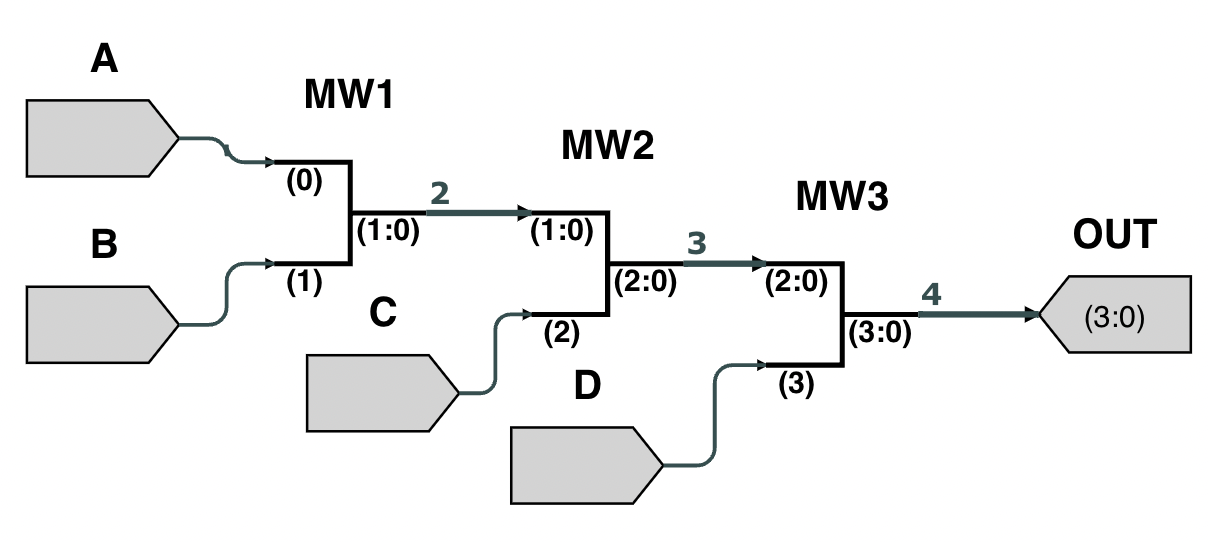
\includegraphics[width=1.0\linewidth]{05.ImpPlan/mergewires.png}
\captionof{figure}{\label{fig:mergewires}Circuit with multiple \textit{MergeWires} connected to each other}
\end{minipage}\hfill %
\begin{minipage}{.45\textwidth}
\begin{equation} \label{equ:longappend}
    OUT = (D::(C::(B::A)))
\end{equation}
\begin{center}
Append as a Binary Operator
\end{center}
\vspace{2em}
\begin{equation} \label{equ:shortappend}
    OUT = D::C::B::A
\end{equation}
\begin{center}
Append as a list of appended expressions
\end{center}
\end{minipage}
\end{center}

\subsubsection{Algebraic Expressions} \label{subsubsec:imp_algebraexps}
Using a DU type, a short grammar was written to represent algebraic expressions in Issie. The grammar writing process in particular validated the choice of F\fsharp as a programming language for the project; the DU type allows for the grammar to be defined succinctly (only 7 lines of code), while pattern matching on DUs enables evaluation of an expression through a single recursive function. Large class hierarchies are therefore not required. Algebraic expressions in Issie are defined by the type \codestyle{FastAlgExp} -- the prefix \textit{Fast} is used as the algebraic expressions are used within the Fast Simulation.

According to the grammar, an algebraic expression (\codestyle{FastAlgExp}) in Issie can be:
\begin{enumerate}
    \item \textbf{\codestyle{SingleTerm of SimulationIO}}: Represents a single algebraic term, which is an input. This case has the type \codestyle{SimulationIO} as every input in Issie is represented by that data structure.
    \item \textbf{\codestyle{DataLiteral of FastData}}: Represents a numeric value in the simulation. 
    \item \textbf{\codestyle{UnaryExp of Op: UnaryOp * Exp: FastAlgExp}}: Represents a unary expression. The unary operator (\codestyle{Op}) takes the expression (\codestyle{Exp}) as its operand. An example would be $-A$.
    \item \textbf{\codestyle{BinaryExp of Exp1: FastAlgExp * Op: BinaryOp * Exp2: FastAlgExp}}: Represents a binary expression, in which a binary operator (\codestyle{Op}), such as '$+$', operates on two expressions. \codestyle{Exp1} is the left operand, \codestyle{Exp2} is the right operand.
    \item \textbf{\codestyle{ComparisonExp of Exp: FastAlgExp * Op: ComparisonOp * uint32}}: Represents a comparison between an algebraic expression (\codestyle{Exp}) and a numeric value.
    \item \textbf{\codestyle{AppendExp of FastAlgExp list}}: Represents an expression that is made up of a group of existing expressions appended together. The list is ordered such that the most significant bit is at the head of the list. F\fsharp lists are are implemented as singly-linked-lists, therefore adding a new item to the head of a list is an $O(1)$ operation. Therefore, having the MSB at the head of the list means that appending something further onto the \codestyle{AppendExp} is efficient.
\end{enumerate}

\subsection{The \codestyle{TableInput} Data Type}
The \codestyle{TableInput} data type is used when generating the input space of the truth table. As discussed in Section \ref{subsec:evolutionofinputspace}, the method for generating a limited input space needs to know exactly which specific input combinations to generate out of potentially billions of possible combinations. To achieve this, a new data structure for representing inputs was required; one which stores more than  the \codestyle{SimulationIO} type. The \codestyle{TableInput} is a record type, and its fields are described by Table \ref{tab:tableinput}.
The term \textit{Row Count} in the context of the input space generation refers to the size of the set ($S_i$) of unique values an input ($x_i$) can contribute to a table.

\begin{table}[!ht]
    \centering
    \begin{tabular}{|m{4cm}|m{9cm}|}
    \hline
        \textbf{Field and Type} & \textbf{Explanation} \\ \hline
        IO: \codestyle{SimulationIO} & Inputs in Issie are represented by the SimulationIO type, which contains the Component ID, Component Label, and the width of the input. \\ \hline
        IsAlgebra: \codestyle{bool} & True if the input is algebraic, as opposed to numeric \\ \hline
        MaxRowCount: \codestyle{int} & The total size of the Set $S_i$, which is equal to $2^{w_i}$, where $w_i$ is the width of the input. \\ \hline
        ConstrainedRowCount: \codestyle{int} & The size of the subset of $S_i$ which contains all input values which conform with the input constraints. For example, if there were the following constraints on the input: $0 \leq x \leq 6$ \& $x = 9$, the Constrained Row Count would be 8. Constrained Row Count is always less than or equal to Max Row Count. \\ \hline
        AllowedRowCount: \codestyle{int} & The number of input values the given input is actually allowed to contribute to the truth table. Ideally, this is equal to the Constrained Row Count, but in situations where the truth table has to be truncated, the Allowed Row Count may be limited to keep the total number of rows in the truth table under the overall limit. \\ \hline
    \end{tabular}
    \caption{Explanation of Fields in the \codestyle{TableInput} data structure}
    \label{tab:tableinput}
\end{table}

\subsection{Table Manipulation Data Types}
The following data types are used in messages sent from the view function to the update function to indicate that some UI interaction has occurred which requires updating certain parts of the model.

\subsubsection{When the Truth Table is out of date}
There are numerous operations a user can perform on a truth table. These range from adding input or output constraints to changing the order of columns. The actions render the displayed truth table out of date. Updating the truth table depends on the action performed as re-generating the table from scratch for all actions would be wasteful and inefficient. Therefore, the update function needs to know exactly which action caused the table to go out of date. This is the purpose of the \codestyle{ReasonOutOfDate} DU type. There are four reasons a truth table may be out of date:
\begin{itemize}
    \item \codestyle{Regenerate}: The truth table needs to be re-generated from scratch. This is due to a change in input constraints or algebraic inputs.
    \item \codestyle{Refilter}: Output constraints have changed, so the truth table needs to be filtered again using the updated constraints.
    \item \codestyle{ReSort}: The IO the table is to be sorted by and/or the order it needs to be sorted in has changed. Sort the table again to reflect this.
    \item \codestyle{HideCol}: An output column has been hidden or unhidden -- change the truth table to reflect this.
\end{itemize}
The circumstances in which these messages are sent, and what exactly happens when they are received will be covered in further detail later in this chapter.

\subsubsection{Truth Table Sorting direction}
\begin{lstlisting}[caption=Definition for Sort Type,frame=tlrb, language=FSharp, label=lst:ttsort]{Name}
type SortType = | Ascending | Descending
\end{lstlisting} 
As shown in Listing \ref{lst:ttsort}, sorting can be done in ascending or descending order.

\subsubsection{Changing the Order of Columns}
\begin{lstlisting}[caption=Definition for Movement Direction,frame=tlrb, language=FSharp, label=lst:ttmovecol]{Name}
type MoveDirection = | MLeft | MRight
\end{lstlisting} 
As shown in Listing \ref{lst:ttmovecol}, columns can be moved left or right.

\section{Top Level UI Changes}
\subsection{Simulation Sub-tabs}
All activities that involved some form of circuit simulation were organised under the \textbf{Simulations} tab (formerly called Simulation) using sub-tabs. The right section tabs are implemented with the Fulma \cite{fulmaio} Tabs component. The Sub-tabs are implemented by nesting a second Fulma Tabs component within the body of the Simulations tab, and making ensuring that a sub-tab is visible only when it and the parent tab is open.

\subsection{Moving the Waveform Simulator}
Due to its inconsistent placement and strange tab-spawning behaviour, the decision was made to move the waveform simulator into its own, permanent sub-tab. The move was quite straightforward; the \textit{Waveforms} button was moved to the sub-tab, a greeting was also displayed. However, one small change had to be made to how the waveform simulator operated. When a waveform simulation is running, other tabs in the app are inaccessible by design. Previously, the waveform simulation tab would only open when the user was either starting or viewing a waveform simulation. Therefore, the existence of the tab was a valid metric for ascertaining whether the app should make other functions inaccessible. Following the changes, however, the existence of the waveform simulation tab is independent of whether a waveform simulation is running. Therefore, a new pair of messages \codestyle{LockTabsToWaveSim} and \codestyle{UnlockTabsFromWaveSim} can be used to control when the user is locked into the Waveform Simulator.

\subsection{Dynamic Dividerbar Resizing}
The dividerbar is situated between the canvas and the right section and marks the boundary between the two. During waveform simulation, the dividerbar becomes draggable to let the user view more content by resizing the right section. This functionality was also extended to truth tables. However, there was a bug in the implementation of the dividerbar. The CSS Style for the dividerbar element sets its height to 100\% of the right section. If the height of the the content in the right section exceeds the initial height of the right section, the latter \textit{overflows} and becomes scrollable. The 100\% height styling on the dividerbar did not take the overflow into account, meaning that the dividerbar would slowly disappear off screen as the user scrolled down. This issue was fixed by getting the right section \codestyle{div} element from the DOM Tree, and reading its \codestyle{scrollHeight}, which takes overflow into account. 

\section{Generating Truth Tables}
Figure \ref{fig:ttGen} in Section \ref{sec:analysis_ttGen} described the high-level method for generating truth tables in Issie. In the interest of consistency for both the user and future developers, as well as ease of maintenance, the truth table generation code either uses the Step Simulator code, or conforms with its design language.



% For only two multi-bit inputs, the library function \codestyle{List.allPairs} \cite{ListFuns} can be used to find this Cartesian product, with each set of possible values being passed in as a List. However, no such library function exists for $n$ sets/lists. The function \codestyle{numbComb} was implemented to find the Cartesian product of $n$ lists. The function is tail recursive for improved performance.




\subsection{Truth Table Generation Algorithm}
\emph{Associated Requirements:} \textbf{E1.1}, \textbf{E1.3}, \textbf{E1.6}


Figure \ref{fig:ttGen} shows a high-level view of the method used to generate truth tables in Issie. The user initiates truth table creation by clicking on a button. Following this, 

As outlined in the previous section, the major hurdle to overcome during truth table generation was the immense size of the input space, as generating and mapping a large input space to its corresponding output space was deemed both inefficient and unnecessary. The final generation algorithm solves this issue by limiting the maximum size the input space can grow to. If the truth table has more input combinations than the limit allows, the truth table is \textbf{truncated}, and only the maximum number of allowed rows are shown. Following some trial-and-error testing, a maximum value of 1024 ($2^10$) rows was chosen. This would allow for small circuits to be wholly represented by the generated truth table, while still allowing for relatively fast truncated truth table generation for larger circuits. The issue with using truncation alone is that the generated truth table does not fully represent the logic. Therefore, users may not be able to find specific rows in the truth table, and conclusions drawn from the truth table may not always be accurate. As a result, the final generation algorithm reduces the input space by \textbf{first applying input constraints, and then truncating if necessary}. If a user generated truth table is truncated, they are warned and it is suggested that they apply more restrictive input constraints to view a specific subset of the truth table.



\subsubsection{Algorithm for generating the Input Space}


\subsection{Numerical Constraints}
\emph{Associated Requirements:} \textbf{E1.5}

As per the requirements, users should have a way of filtering the truth table by applying numerical constraints to table inputs and outputs. This is necessary to reduce the size of the table and allow users to analyse relationships between inputs and outputs for a subset of the input space. 


% \subsubsection{Visualising Truth Tables}
% As of the Interim report, Truth Tables are visualised using Fulma Tables. They are clear, responsive and do a good job overall. However, they lack interactivity. Therefore, it is anticipated that they will be replaced or modified in the future. For viewing multi-bit inputs and outputs, hexadecimal was chosen over binary as it would take up less physical space. Currently, there is no option to change number base (as there is in the Step Simulator), but this would be trivial to implement in the future. Truth Table generation and viewing is done in an MVU way; pressing the "Generate Truth Table" button causes a truth table to be generated and stored in the \textbf{Model} through a message which is processed by the \textbf{Update} function. On the next call of the View function, this Truth Table is rendered.


\subsection{Generating Truth Tables for a partial selection of a Sheet}
\emph{Associated Requirements:} \textbf{E1.2}, \textbf{E1.3}

% The motivation behind Requirement \textbf{E1.2} is that a large schematic with lots of components will often contain smaller blocks of logic within it. These blocks may be defined Custom Components, or simply be a collection of gates in one corner of the canvas. Either way, there is value in the user being able to isolate these blocks and learn about the combinational logic implemented by them. Such functionality would also allow users to take a divide-and-conquer approach to debugging logical errors - individual blocks could be inspected to ascertain if they had been implemented correctly. 

% A challenge with generating a truth table from part of a canvas is that Issie has no existing method for simulating part of a canvas. When working with a whole sheet, the inputs and outputs are well-defined; sheets where any ports aren't connected to inputs/outputs throw \textit{Simulation Errors}. In contrast, a partial selection from a sheet will rarely contain all inputs and outputs. Two methods were considered for simulating the selected logic to generate a truth table, with the latter being chosen.
% \begin{enumerate}
%     \item \textbf{Extracting the Fast Simulation and feeding values into specific wires}. This method would have involved creating a Fast Simulation for the whole sheet as usual, but then manually changing values in component arrays and seeing how those changes propagated through to the output connections of the selected logic. While this method seemed fit initially, several issues were found after some analysis. The Fast Simulation would be built for the whole sheet, meaning that an error elsewhere on the canvas would stop the selected logic from being simulated. Custom Components would also be harder to manage as the Fast Simulation datatype flattens the design, meaning that all nested logic in Custom Components would be expanded out. The new logic would also be quite different from the truth table generation logic for whole sheets - this is not ideal for future code maintenance purposes.
%     \item \textbf{Intelligently building and correcting a new Canvas}. Following the highlighting of the issues with the first approach, an alternative approach was put forward. Rather than attempting to work with the complicated Fast Simulation data structure, it instead aims to use as much of the existing code as possible by treating the selected logic as a separate instance of a Canvas State and trying to simulate it using the same method as simulating a whole canvas. The main difference between simulating a whole sheet and simulating selected logic is the lack of guaranteed input and output components. This is overcome by finding which ports/connections are inputs/outputs for the selected logic, then intelligently adding 'phantom' input/output components to the canvas in a process called Canvas Correction. Once a corrected canvas corresponding to the selected logic is created, the logic used for generating and viewing a Truth Table for a whole sheet can be reused.
% \end{enumerate}

% Prior to the canvas correction stage, the selected components are checked. If only connections are selected, then a \textit{Simulation Error} is returned to the user informing them of their mistake.

\subsubsection{Canvas Correction}
\begin{itemize}
    \item[Step 1] \textbf{Add Extra Connections:} Sub-figures \ref{subfig:SelCase2} to \ref{subfig:SelCase4} in Figure \ref{fig:SelCases} all show situations where one or more inputs/outputs for the selected logic are ports on components, rather than connections. Taking the case shown in Figure \ref{subfig:SelCase2} in particular, the inputs to the selected logic are: both input ports on G1, and the bottom input port on G2, while the outputs from the selected logic are both output ports on G1 and G2 respectively. Prior to correction, the selection canvas does not have any connections going into those ports. This step finds any ports on selected components which do not have a connection in the selection and connects them to "dummy" input or output ports depending on their \codestyle{PortType}. This transforms the canvas to a state similar to that seen in Case (a), where   all inputs into the selected logic have connections.
    \item[Step 2] \textbf{Add Extra IOs:} This step adds the "phantom" input and output components to the selection canvas. The locations where these components need to be inserted are found by checking which connections in the Canvas State do not have both ports present in the selection. Any such connections are either connected to some other component in the sheet which is not selected, or are newly added connections which are connected to dummy ports. Either way, these are the connections that need to be connected to "phantom" IOs. 
    \begin{itemize}
        \item[Step 2.1] \textbf{IO Width Inference:} When creating new input or output components, the correct width must be specified. This is         calculated by running Issie's \codestyle{WidthInferrer} on the whole sheet to find the expected width of the input or output. However, in cases such as the one shown in Figure \ref{subfig:SelCase4}, where there are no connections to/from some ports on G3, \codestyle{WidthInferrer} will fail to infer widths, resulting in a \textit{Simulation Error}. A possible workaround would be to try to infer the width from the component itself if \codestyle{WidthInferrer} fails - in Issie AND gates always have 1-bit inputs, so any "phantom" inputs generated would have a width of one. This would be trivial to implement in the future. However, there would still be cases, such as inputs into multiplexers and n-bit XORs, where even this approach would not work.
        \item[Step 2.2] \textbf{IO Label Inference:} Usually users provide labels for IOs, which are used in the Truth Table. However, when IOs are automatically created, names for them must be automatically generated too. This is done by looking at which ports in the selection they are connected to. The expression for an automatically generated IO Label is: \codestyle{[Connected Component Label]\_[IN/OUT][SUFFIX]}. If the port is labelled (e.g. on a multiplexer or a Custom Component), the suffix is the port label. Alternatively it is the \codestyle{PortNumber}, which indicates the position of a port on its host component.
        
    \end{itemize} 
    \item[Step 3] \textbf{Returning a Canvas or an Error:} If any errors were found in the previous steps, most likely due to a malformed selection, they are returned. If not, then the returned Canvas State is completely compatible with the existing simulation and truth table generation functions.
\end{itemize}

Following Canvas Correction, any returned Canvas State is fully compatible with the existing functions for simulating logic and generating truth tables. Therefore, a Truth Table can be generated for selected logic through the same methods and functions used for generating Truth Tables for the whole sheet.

\bigskip
\begin{figure} [h]
    \begin{subfigure}{0.48\textwidth}
        \centering
        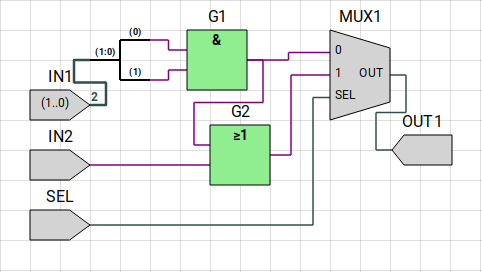
\includegraphics[width=0.8\linewidth]{05.ImpPlan/SelCase1.png}
        \caption{Case where all inputs into selected logic are connections.}
        \label{subfig:SelCase1}
    \end{subfigure}
    \begin{subfigure}{0.48\textwidth}
        \centering
        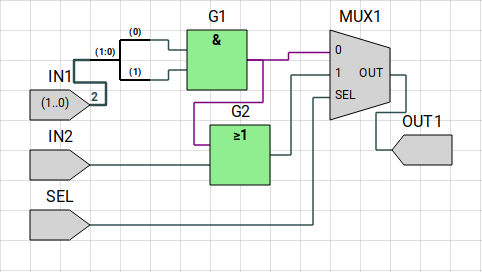
\includegraphics[width=0.8\linewidth]{05.ImpPlan/SelCase2.png}
        \caption{Case where some inputs into selected logic are connections, and some are ports on components.}
        \label{subfig:SelCase2}
    \end{subfigure}
    \newline
    \begin{subfigure}{0.48\textwidth}
        \centering
        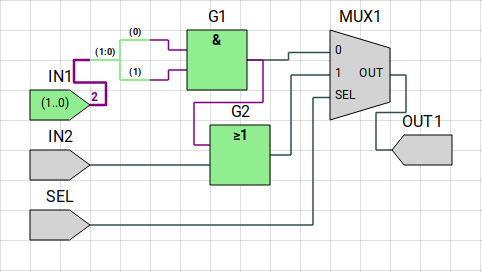
\includegraphics[width=0.8\linewidth]{05.ImpPlan/SelCase3.png}
        \caption{Case where selected logic includes an input component.}
        \label{subfig:SelCase3}
    \end{subfigure}
    \begin{subfigure}{0.48\textwidth}
        \centering
        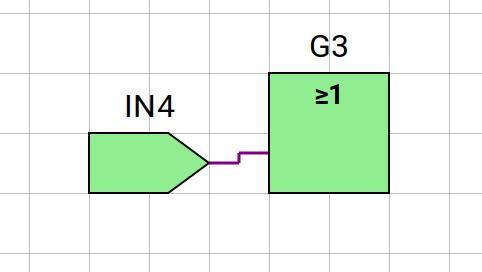
\includegraphics[width=0.8\linewidth]{05.ImpPlan/SelCase4.png}
        \caption{Case where a selected component does not have connections to all ports}
        \label{subfig:SelCase4}
    \end{subfigure}
    \caption{Selection Cases}
    \label{fig:SelCases}
\end{figure}

\subsection{UI Changes}
\emph{Associated Requirements:} \textbf{D3.1}
As mentioned in Section \ref{sec:IssieUI}, there are inconsistencies in Issie's current UI, particularly concerning the Waveform Simulator. With the addition of Truth Table viewing to Issie, the decision was made to tweak the UI to try to keep everything consistent. Figures \ref{fig:OldUI} and \ref{fig:NewUI} show the old and newly tweaked UIs respectively. The top bar primarily houses operations or information concerning files, such as the button to save the sheet, menu to open other sheets/projects, and the filepath. As a result the \textit{Waveforms} button has been removed from there. Ideally it would have a permanent place on the right tab, however with the addition of a Truth Table tab this would take the total number of tabs up to five, causing the tab label text to become illegible.  Given that there are now three ways to gain an insight into the logic on the sheet (Step Simulator, Truth Tables, Waveform Simulator), it is logical to group these together as sub-tabs under one main tab. The new UI now always has three tabs on the right in contrast to the old UI which would spawn the WaveSim tab when viewing Waveforms. Clicking the right-most "Simulations" tab will now reveal three sub-tabs: Step Simulation, Truth Tables, and Wave Simulation. The behaviour of the Truth Table view and the updated WaveSim view is modelled on that of the Step Simulator. Selecting a tab for the respective simulator will reveal a short description of the function, and a button to start the appropriate action. The colour and message shown by this button is dependent on the sheet: problems will show a yellow button, and a solid green button shows that the sheet is correct, and the functionality is available. Light green means that while the sheet is syntactically correct, some other factor is making the functionality unavailable. For the Waveform simulator this is when the sheet contains no synchronous logic (meaning no waveforms to display), and for Truth Tables it is when the sheet does contain synchronous logic (as synchronous logic is currently not supported for truth tables).

\begin{figure}
    \centering
    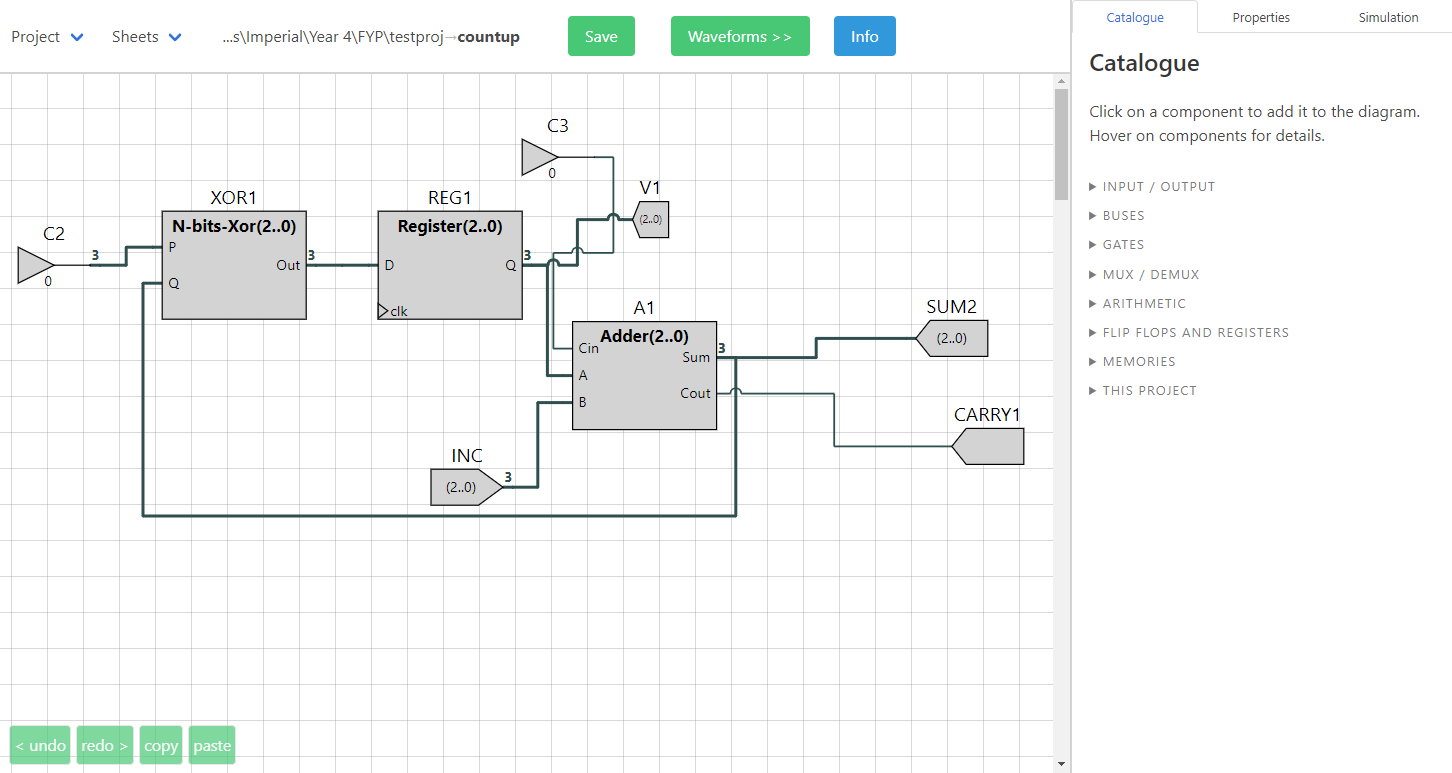
\includegraphics[width=0.8\textwidth]{05.ImpPlan/OldUI.png}
    \caption{Old Issie UI}
    \label{fig:OldUI}
\end{figure}

\begin{figure}
    \centering
    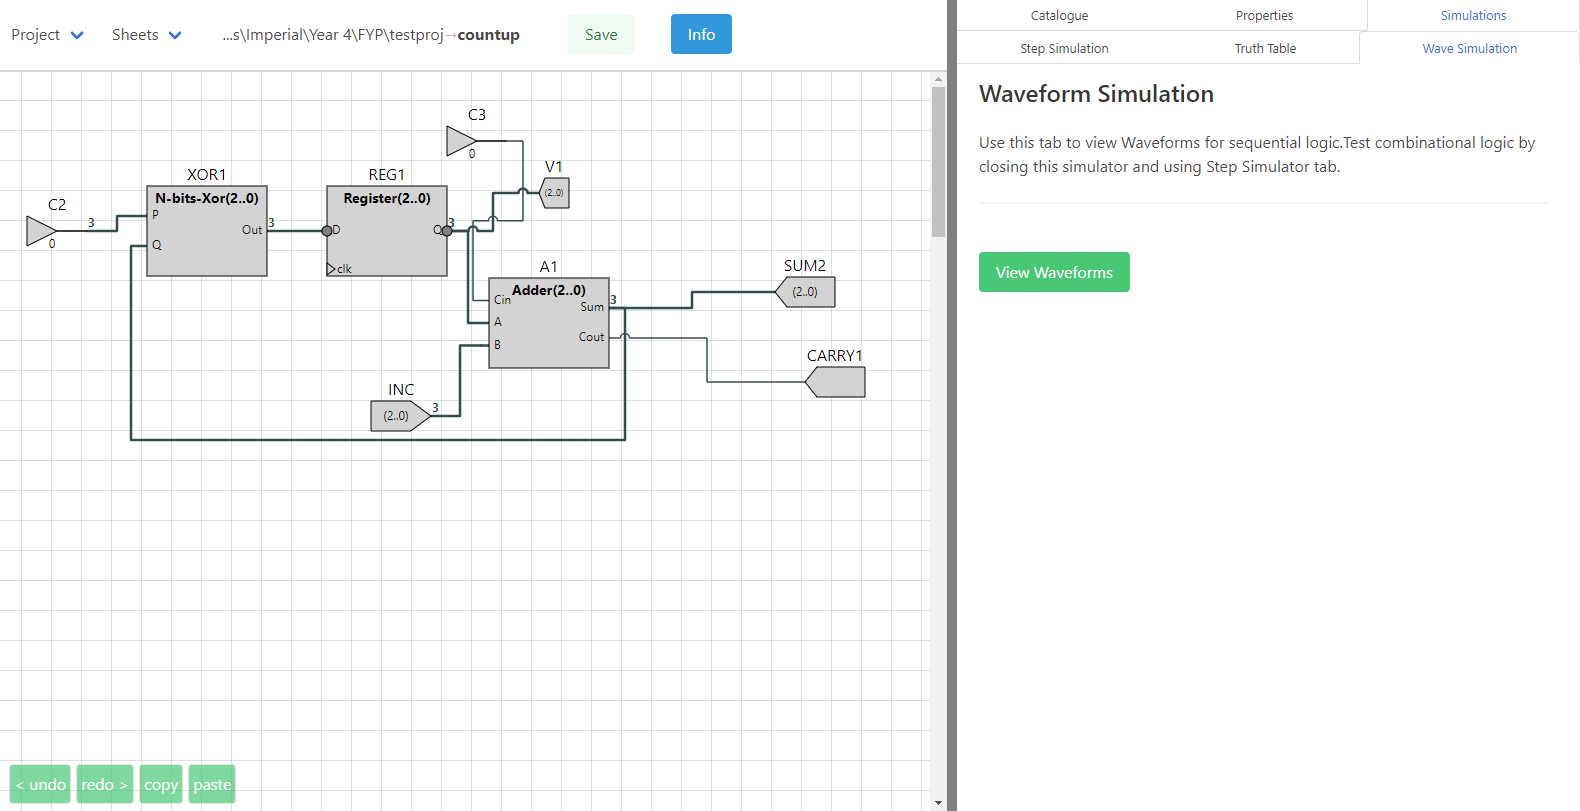
\includegraphics[width=0.8\textwidth]{05.ImpPlan/NewUI.png}
    \caption{New Issie UI}
    \label{fig:NewUI}
\end{figure}

\section{Work Breakdown Structure}
As with any large project, a key stage in planning is to break it down into several manageable chunks. This has been done to some extent in the Requirements Capture (Chapter \ref{chap:requirements}), albeit at quite a high level. On the other hand, a Work Breakdown Structure (WBS) \cite{projectmanagement} defines the scope of the project and breaks the work down into components that can be scheduled, monitored, and controlled. This aids in assessing the complexity of certain tasks, therefore improving the overall distribution of resources (mainly time) to different tasks. The WBS for this project is shown in Figure \ref{fig:wbs} - it is rotated to make it more clear to the viewer. Red nodes in the WBS could be considered as \emph{Initiatives}, as they are long term (relative to the length of the project) objectives. Green nodes are rough equivalents to \emph{Epics}, and white/grey nodes are \emph{User Stories}. In some cases, user stories may have very short sub-tasks underneath them which need not necessarily be differentiated, but are done on the WBS for clarity's sake. User Stories which spawn sub-tasks are coloured purple, while sub-tasks requiring further elaboration are coloured yellow. 

\section{Time Management and Gantt Chart}
Effective time management is vital to any project; traditionally a Gantt chart is used to display the timeframe in which the tasks detailed in the WBS will be completed. In line with this, a Gantt chart has been prepared for this project, and can be seen in Figure \ref{fig:gantt}. The colour coding on the chart matches that on the WBS, and key deadlines are indicated by dashed vertical lines. The first line represents the Interim report deadline - therefore any work shown on the chart to the left of this line is already completed, while any work to the right of the line is planned. The layout of Figure \ref{fig:gantt} allows it to double as a chronologically structured backlog. Within Initiatives, Epics are placed in chronological order, and likewise for User Stories within Epics. Two main considerations were made when devising this order of items. Firstly, dependencies were considered - for example it would be foolish to write code to view truth tables prior to there being a mechanism to generate them. Secondly, the importance of the deliverable associated with a task was taken into account - with tasks that fulfilled essential requirements given precedence over those that fulfilled desired requirements. 

\subsection{Contingencies and Strategies taken to Mitigate Risk}
The project plan has been structured to contain a healthy contingency allowance. Looking at the order of work in the Gantt chart, it can be seen that all essential requirements (and the majority of the desired features) should be fulfilled by the beginning of May. Furthermore, all technical work is expected to be completed by the end of May, bar a possible need to reconfigure parts of Issie's overall GUI (which is very unlikely).
Additionally, most time estimations for tasks have some margin built in as well, reducing the likelihood of technical work overrunning. This leaves the last three weeks of the project dedicated solely to report writing and documentation; two tasks which ideally will have been worked on over the duration of the project. Therefore, this plan yields a contingency allowance of three weeks.
The project management strategy, formed by a fusion of plan-based and Agile management methods, also acts as a form of contingency. As stated, the backlog ordering methodology has taken into account dependencies and importance of deliverables. If progress is slow, then the backlog can be dynamically reorganised, with less essential items shifted or removed. The ultimate fallback is to only implement the essential features, but such an extreme case is highly unlikely to arise. On the other hand, if progress runs ahead of schedule extension tasks can be discussed.

\begin{figure}
    \centering
    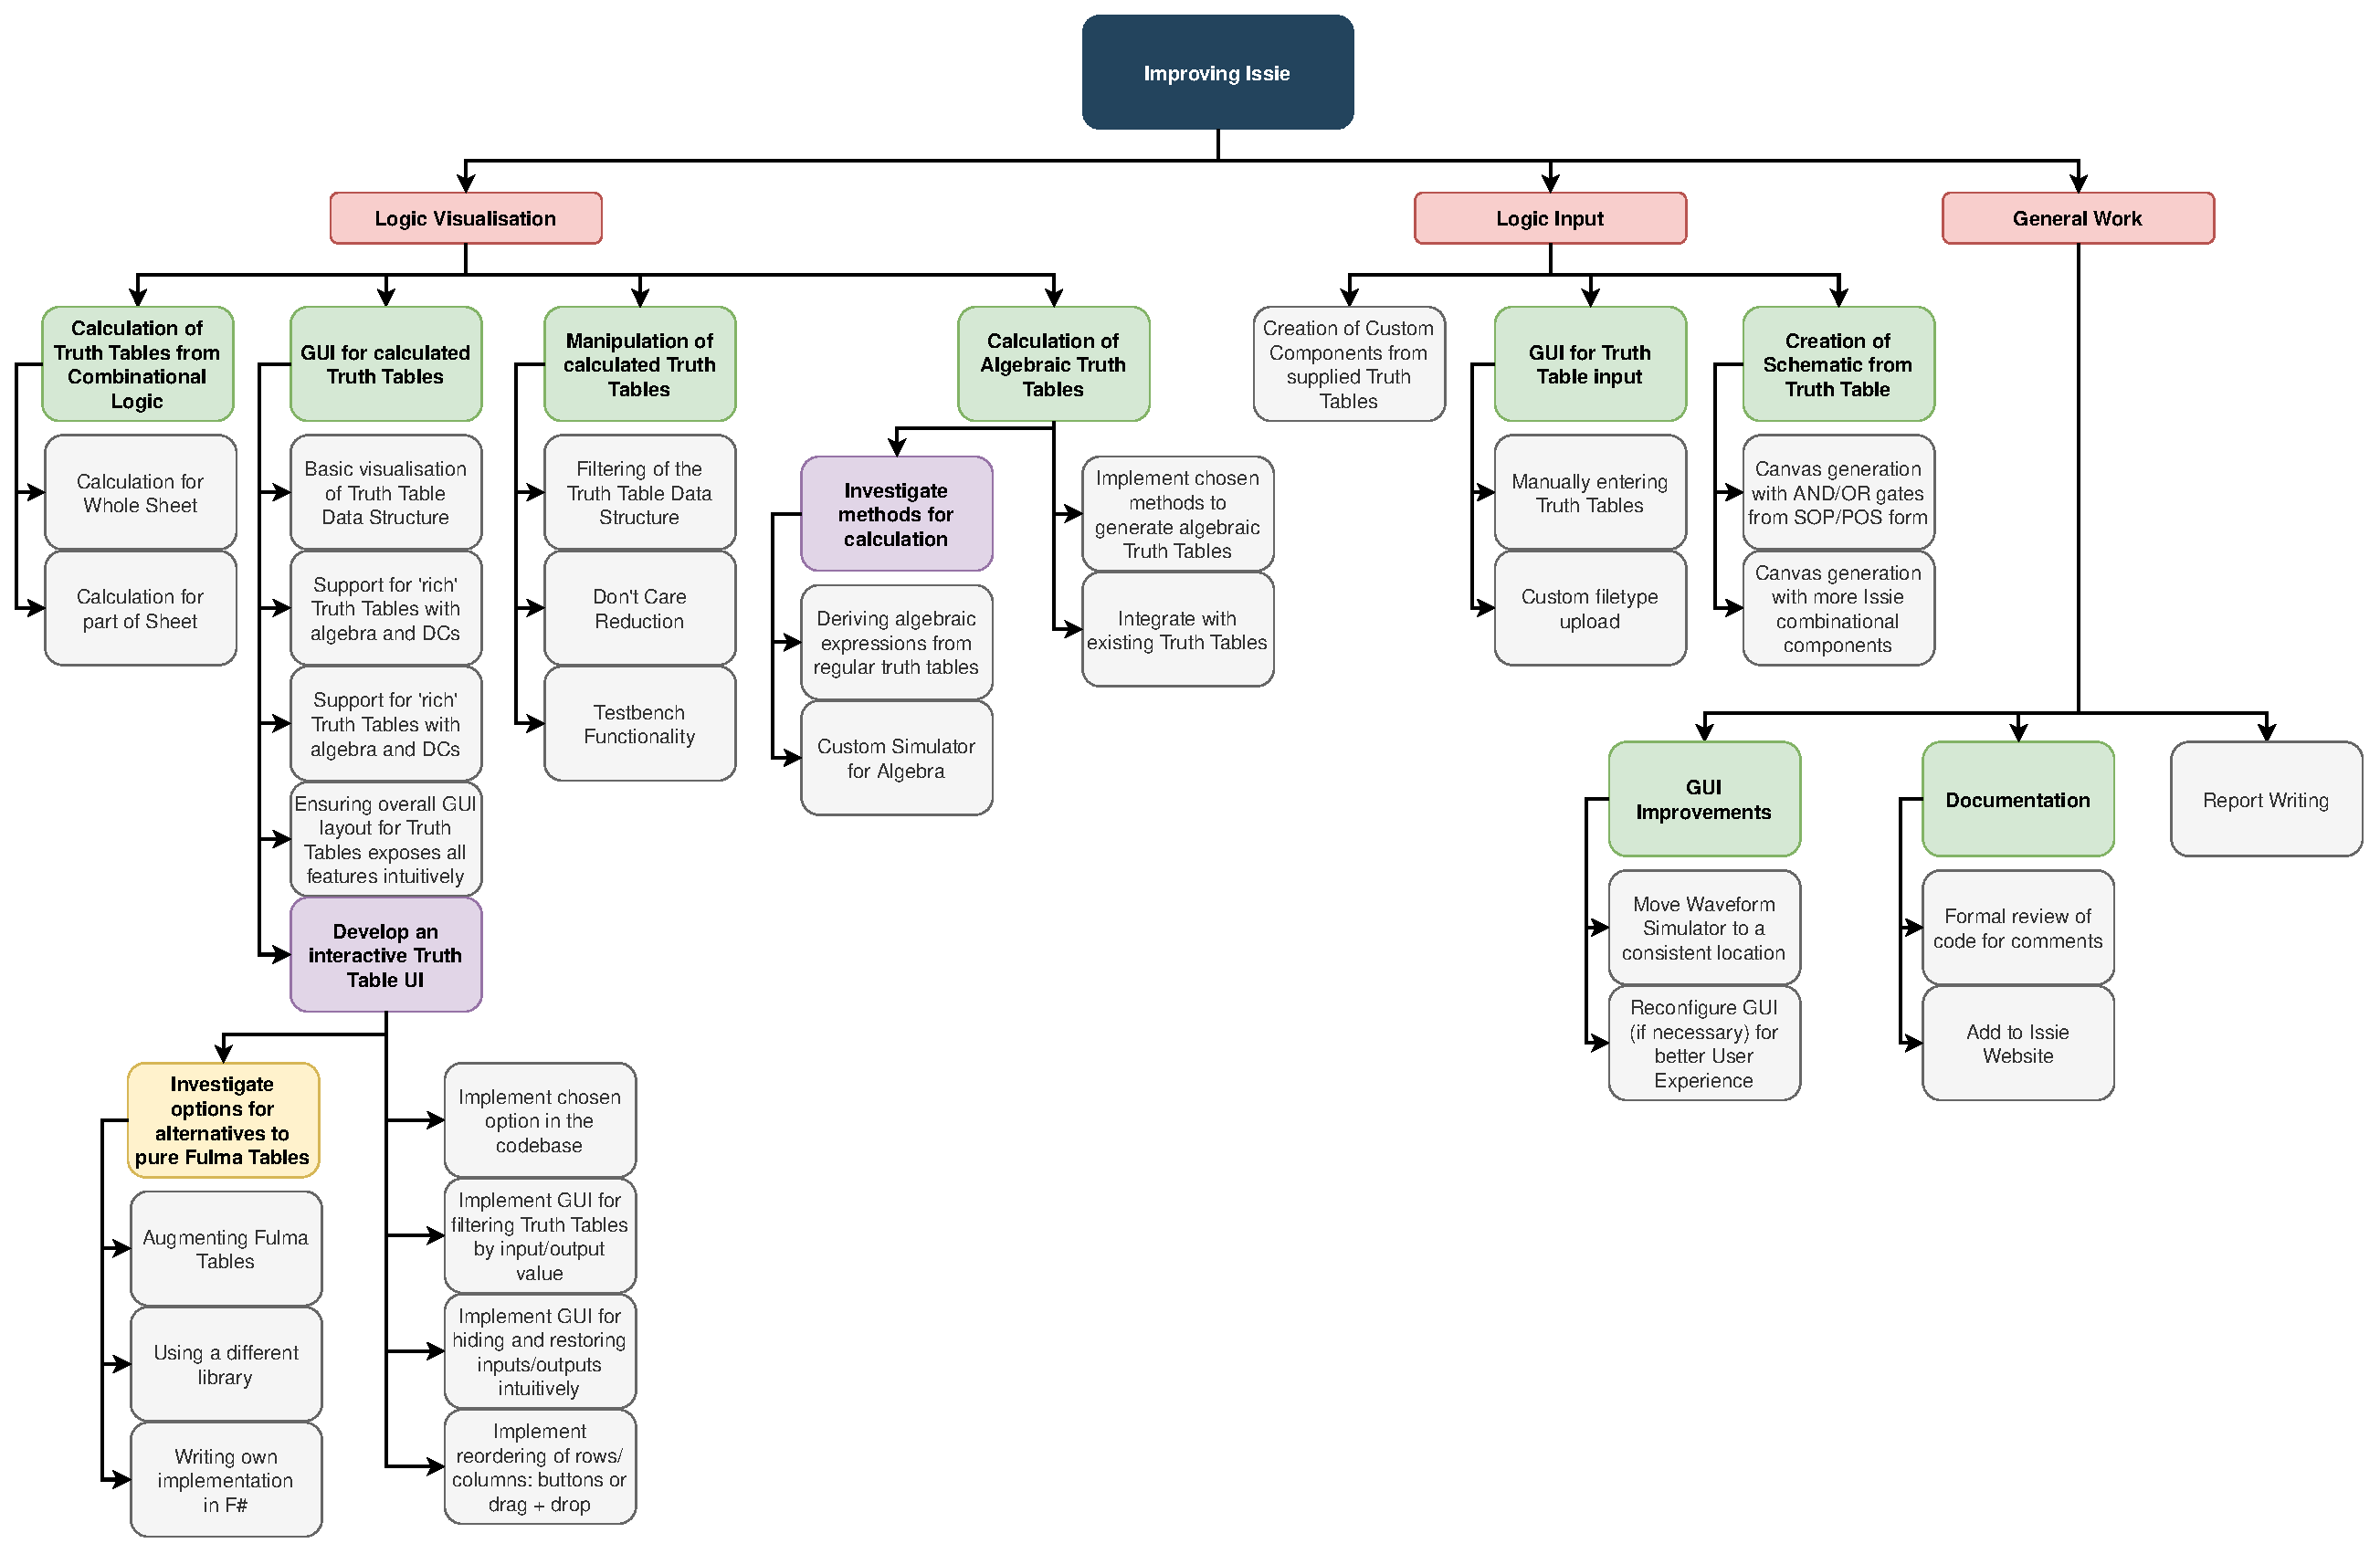
\includegraphics[width=22cm,angle=270,origin=c]{05.ImpPlan/wbs.eps}
    \caption{Work Breakdown Structure for the Project (Rotated)}
    \label{fig:wbs}
\end{figure}

\begin{figure}
    \centering
    \includegraphics*[width=\textwidth]{05.ImpPlan/gantt_update.pdf}
    \caption{Gantt Chart for the Project}
    \label{fig:gantt}
\end{figure}